%-----------------------------------LICENSE------------------------------------%
%   This file is part of Mathematics-and-Physics.                              %
%                                                                              %
%   Mathematics-and-Physics is free software: you can redistribute it and/or   %
%   modify it it under the terms of the GNU General Public License as          %
%   published by the Free Software Foundation, either version 3 of the         %
%   License, or (at your option) any later version.                            %
%                                                                              %
%   Mathematics-and-Physics is distributed in the hope that it will be useful, %
%   but WITHOUT ANY WARRANTY; without even the implied warranty of             %
%   MERCHANTABILITY or FITNESS FOR A PARTICULAR PURPOSE.  See the              %
%   GNU General Public License for more details.                               %
%                                                                              %
%   You should have received a copy of the GNU General Public License along    %
%   with Mathematics-and-Physics.  If not, see <https://www.gnu.org/licenses/>.%
%------------------------------------------------------------------------------%

%   Use the standalone class for displaying the tikz image on a small PDF.
\documentclass[crop, tikz]{standalone}

%   Import the tikz package to use for the drawing.
\usepackage{tikz}

%   Load the arrows.meta library.
\usetikzlibrary{arrows.meta}

%   Begin the document.
\begin{document}
    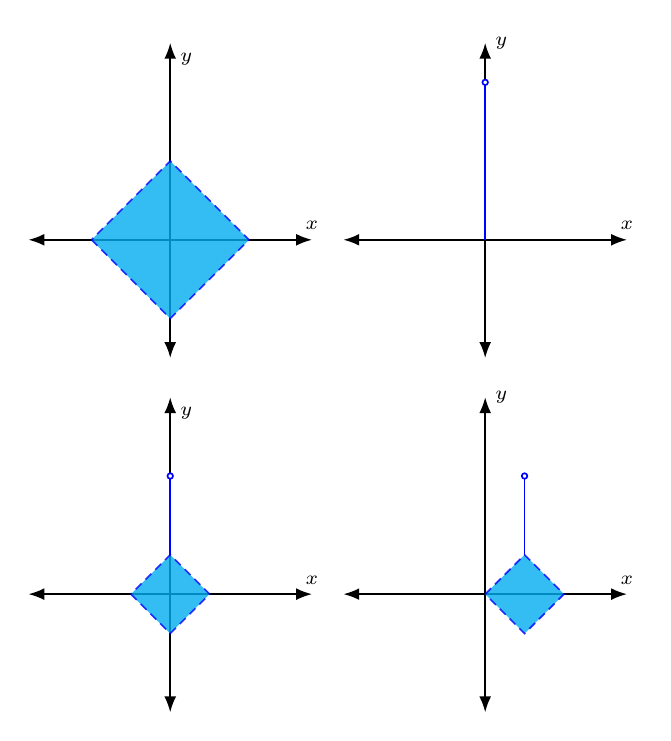
\begin{tikzpicture}[>=Latex,semithick,draw=blue,font=\scriptsize]
        % Draw the first open ball.
        \draw[<->,draw=black] (-1.8,0) -- (1.8,0)
            node [above] {$x$};
        \draw[<->,draw=black] (0,-1.5) -- (0,2.5)
            node [below right] {$y$};
        \draw[fill=cyan,opacity=0.8,densely dashed]
            (-1,0)--(0,-1)--(1,0)--(0,1)--cycle;

        % Draw the second open ball.
        \draw[<->,draw=black] (2.2,0) -- (5.8,0)
            node [above] {$x$};
        \draw[<->,draw=black] (4,-1.5) -- (4,2.5)
            node [right] {$y$};
        \draw (4,0)--(4,2);

        % Draw the third open ball.
        \begin{scope}[yshift=-4.5cm]
            \draw[<->,draw=black] (-1.8,0) -- (1.8,0)
                node [above] {$x$};
            \draw[<->,draw=black] (0,-1.5) -- (0,2.5)
                node [below right] {$y$};
            \draw[fill=cyan,opacity=0.8,densely dashed]
                (-0.5,0)--(0,-0.5)--(0.5,0)--(0,0.5)--cycle;
            \draw (0,0.5)--(0,1.5);
        \end{scope}

        % Draw the fourth open ball.
        \begin{scope}[xshift=4cm,yshift=-4.5cm]
            \draw[<->,draw=black] (-1.8,0) -- (1.8,0)
                node [above] {$x$};
            \draw[<->,draw=black] (0,-1.5) -- (0,2.5)
                node [right] {$y$};
            \draw[fill=cyan,opacity=0.8,densely dashed]
                (0,0)--(0.5,0.5)--(1,0)--(0.5,-0.5)--cycle;
            \draw (0.5,0.5)--(0.5,1.5);
        \end{scope}

        % Draw nodes indicating which points are not included.
        \begin{scope}[
            every node/.style={
                circle,
                fill=white,
                draw=blue,
                inner sep=0pt,
                minimum size=2pt
            }
        ]
            \node at (4,2) {};
            \node at (0,-3) {};
            \node at (4.5,-3) {};
        \end{scope}
    \end{tikzpicture}
\end{document}
